\documentclass[a4paper]{scrartcl}
\usepackage[ngerman]{babel}
\usepackage[utf8]{inputenc}
\usepackage{geometry}                		             		
\usepackage{graphicx}
\usepackage{amsmath}										
\usepackage{amssymb}
\usepackage{subfigure}
\setkomafont{sectioning}{\bfseries}	

\title{Widerstandsmessung am Halbleiter}
\author{Nora Salgo, Manuel Sommerhalder, Fabian Stäger}
		
\begin{document}
\begin{titlepage}
	\centering
	
\includegraphics[width=0.5\textwidth]{uzh.png}\par\vspace{1cm}
	\vspace{1cm}
	{\Large Praktikumsbericht Festkörperphysik\par}
	\vspace{1.5cm}
	{\huge\bfseries Widerstandsmessung am Halbleiter\par}
	\vspace{2cm}
	{\Large\itshape Nora Salgo, Manuel Sommerhalder, Fabian Stäger \par\vspace{1cm}
	Assistent: Kay Waltar}
	\vfill
	

	\vfill

% Bottom of the page
	{\large \today\par}
\end{titlepage}

\section{Aufbau}

\subsection{Thermoelement}
Ein Thermoelement besteht aus einem Stromkreis mit zwei verschiedenen Metallen A und B. Wenn zwischen den Kontaktstellen eine Temperaturdifferenz existiert, entsteht gemäss dem Seebeck-Effekt eine elektrische Spannung 
$$ U = \int_{T_{1}}^{T_{2}} S_{B}(T) - S_{A}(T) \, dT $$
wobei die Seebeck-Koeffizienten $S_{A}$ und $S_{B}$ temperaturabhängige Materialeigenschaften mit der Einheit V$/$K sind. Mithilfe einer Spannungstabelle (siehe Anhang auf Seite \pageref{Kacktabelle}) kann der gemessenen Spannung eine Temperatur zugeordnet werden. In diesem Experiment wurde ein NiCr-Ni-Thermoelement verwendet.

\subsection{Vierpunkt-Widerstandsmessung}
Um den Widerstand der Probe möglichst genau zu messen, wird die Vierpunkt-Methode verwendet. Dabei fliesst über zwei der Leitungen ein bekannter Strom durch den Widerstand. Der Spannungsabfall am Widerstand wird über zwei weitere Leitungen abgegriffen. Der Widerstand kann dann mithilfe des Ohmschen Gesetzes berechnet werden.


\newpage

\section{Messdaten}

\subsection{Temperaturverlauf}
Während des Versuchs wurde die Temperatur in der Heizspule und an der Probe gemessen. In Figur \ref{temp_time} ist ersichtlich, dass die Probentemperatur der Reglertemperatur im Aufwärmprozess hinterherhinkt. Für die Auswertung wird nur die Probentemperatur berücksichtigt.
%
\begin{figure}[htbp]
\centering
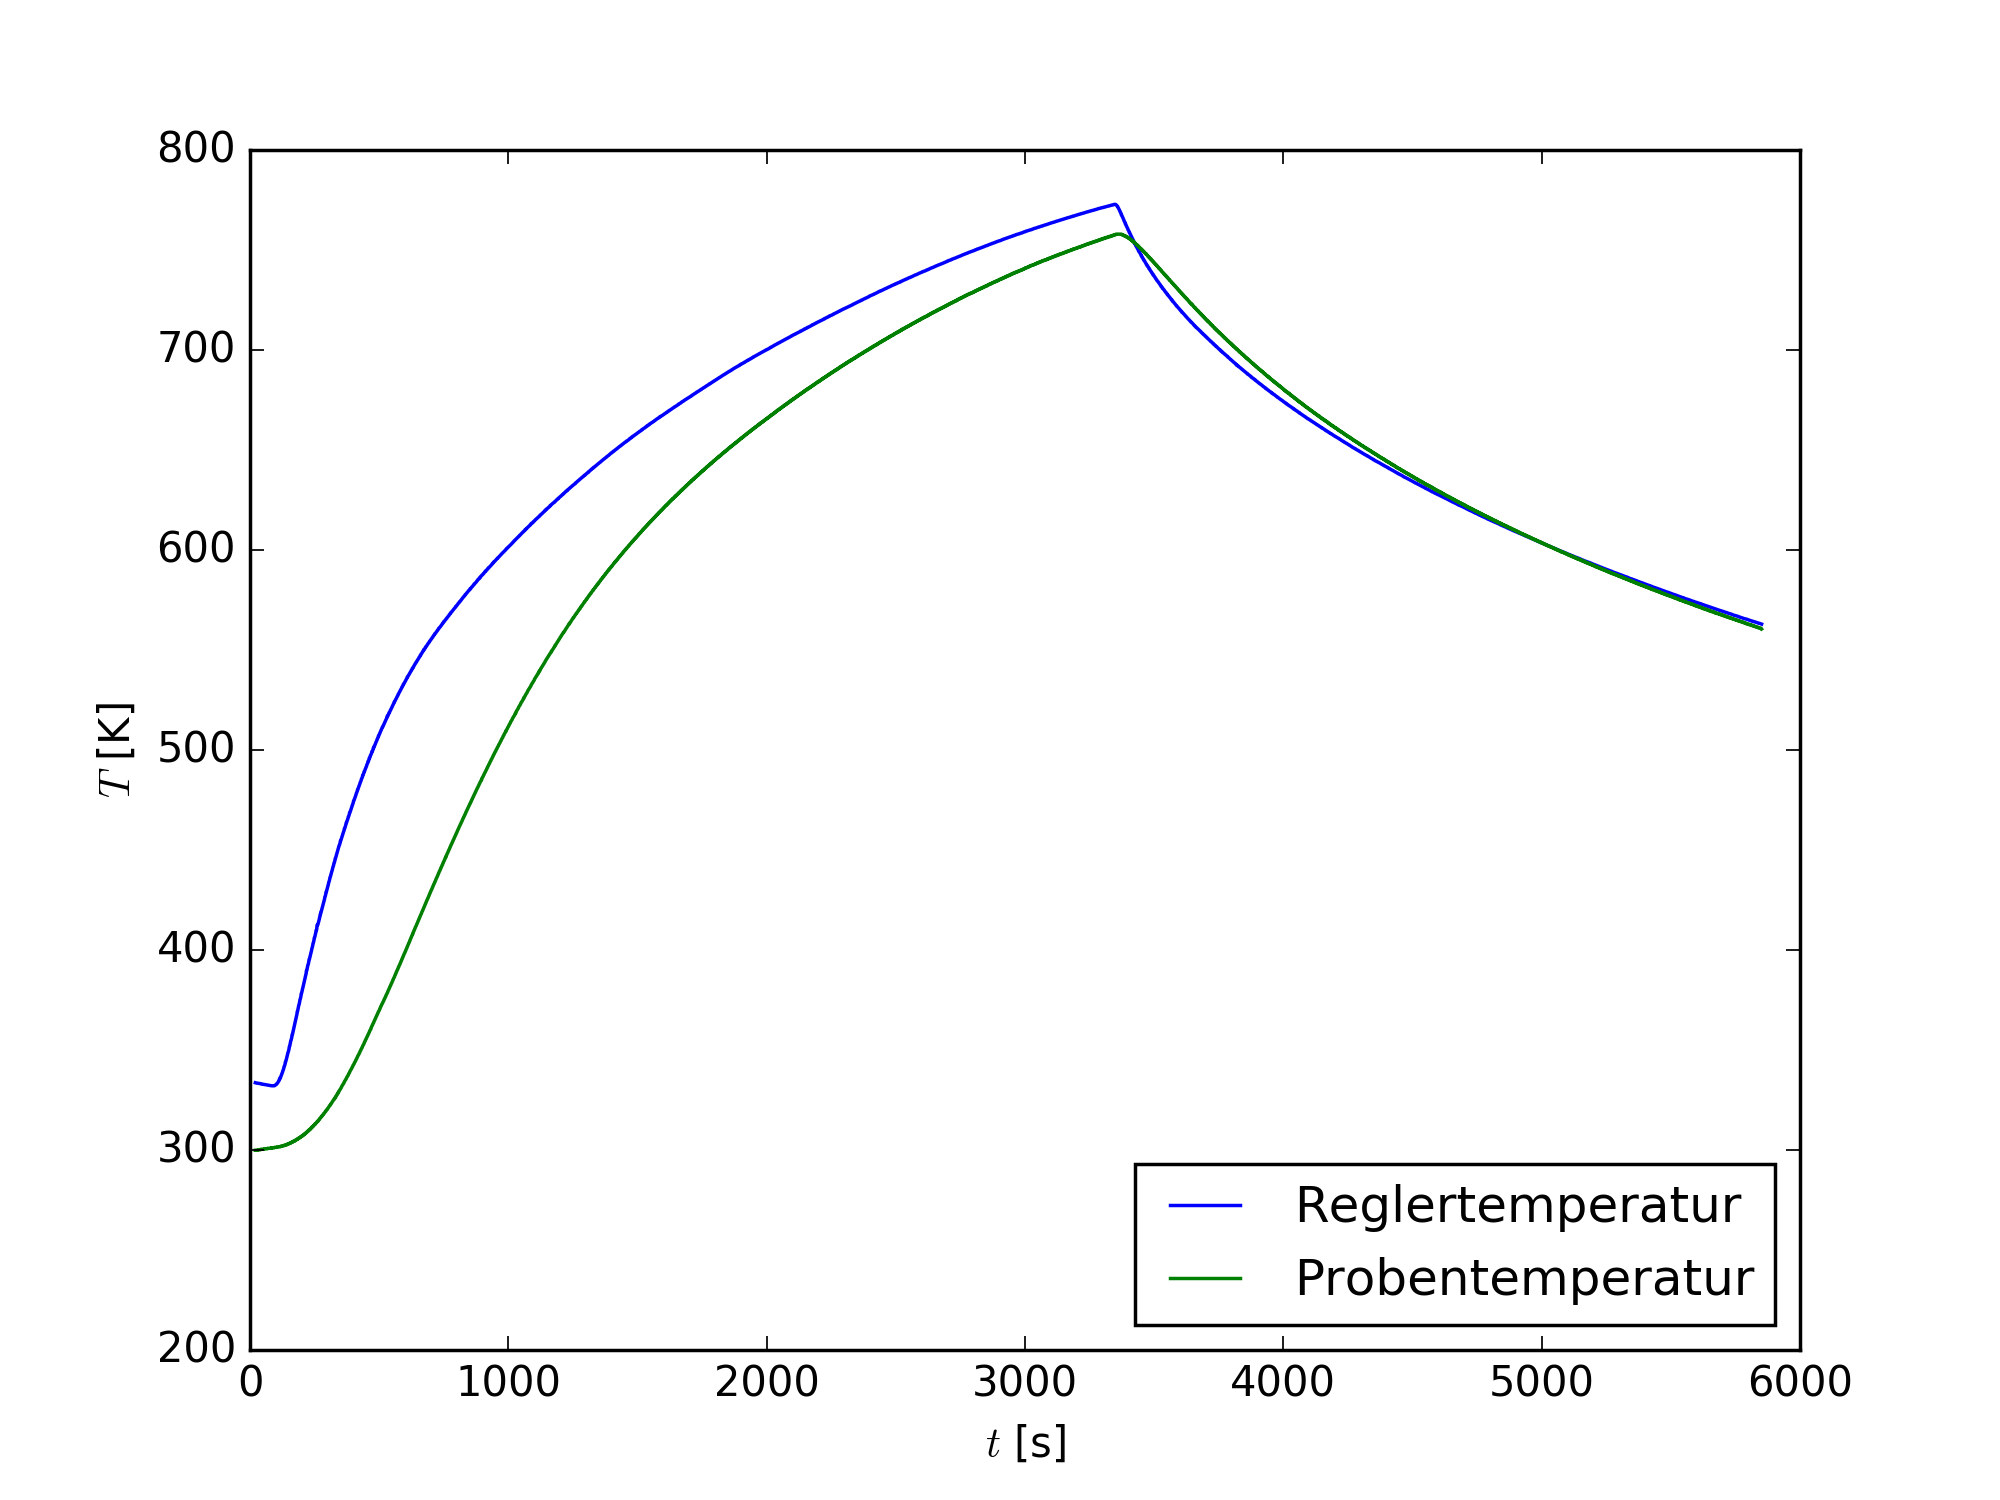
\includegraphics[width=0.9\textwidth]{temp_time.png}
\caption{Temperaturverlauf über die Zeit}
\label{temp_time}
\end{figure}
%

\subsection{Temperaturabhängigkeit des elektrischen Widerstands}
Die Siliziumprobe wurde zuerst auf $500^{\circ}$C erwärmt und dann wieder auf Raumtemperatur abgekühlt. Während des ganzen Prozesses wurde der elektrische Widerstand mit der Vierpunkt-Messmethode ermittelt. In der Skizze (Abbildung \ref{res_temp}) ist ersichtlich, dass der Widerstandsverlauf bei Aufwärm- (blau) und Abkühlprozess (grün) leicht unterschiedlich ausfällt.
%
\begin{figure}[htbp]
\centering
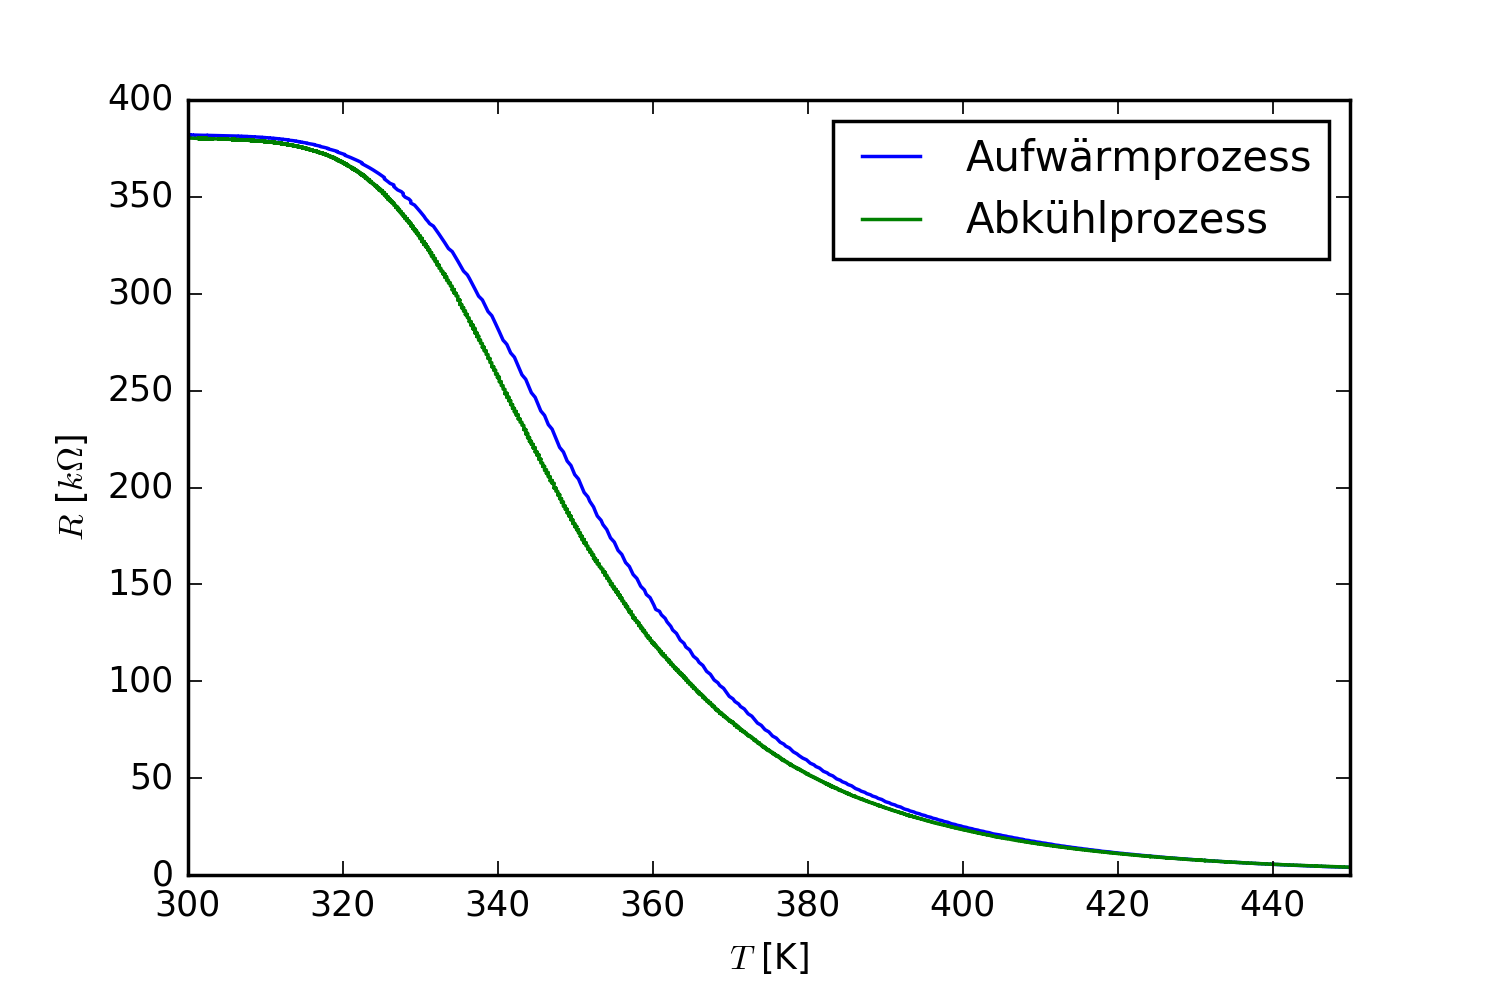
\includegraphics[width=0.9\textwidth]{res_temp.png}
\caption{elektrischer Widerstand des Halbleiters}
\label{res_temp}
\end{figure}
%

\newpage
\section{Appendix}
\subsection{Spannungstabelle Thermoelement}
\label{Kacktabelle}
\begin{figure}[htbp]
\centering
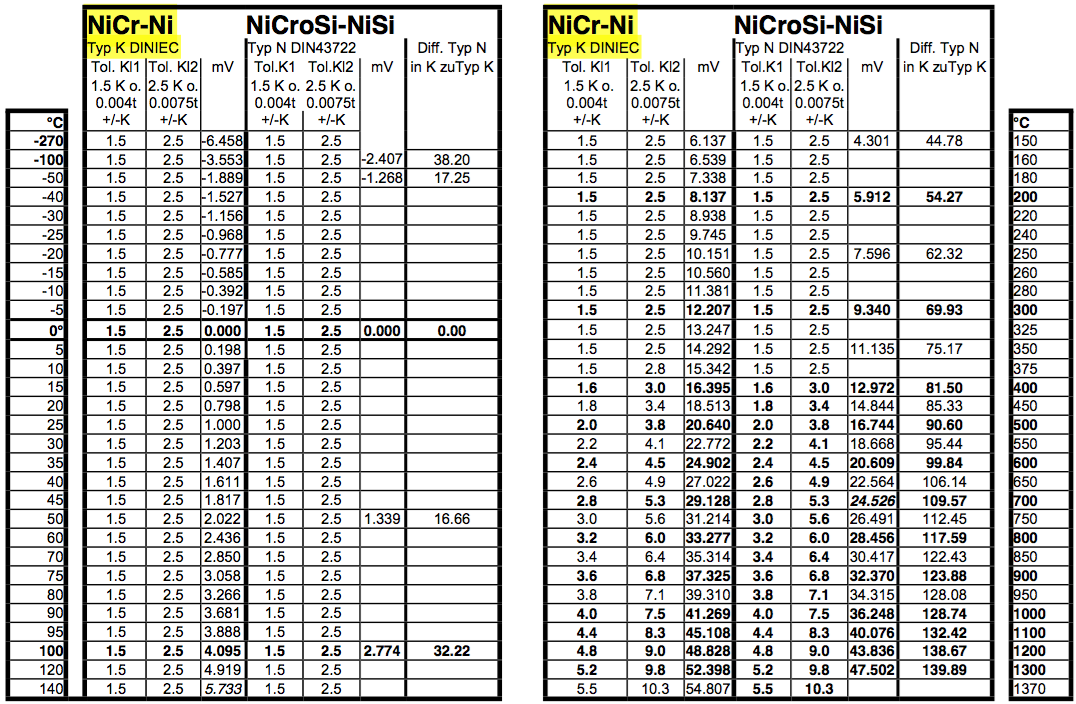
\includegraphics[width=1\textwidth]{spannungstabelle.png}
\label{temp_cool}
\end{figure}
%
Als Bezugspunkt wird in dieser Tabelle die Vergleichsstellentemperatur $T_{0}=0^{\circ}C$ verwendet. Für die Messung bei Raumtemperatur $T_{R} \approx 26^{\circ}C$ muss dies entsprechend kompensiert werden:
$$ U_{th} = U_{1} \, (1-\frac{T_{0}}{T_{R}}) $$






\end{document}  